\documentclass[border=4pt]{standalone}
\usepackage{graphicx,xcolor,tikz}
\usetikzlibrary{arrows.meta,positioning,fit,calc,backgrounds}
\pgfdeclarelayer{bg}
\pgfsetlayers{bg,main}
\definecolor{colA}{RGB}{44,100,170}
\definecolor{colB}{RGB}{178,72,72}
\definecolor{colC}{RGB}{35,139,69}
\definecolor{colH}{RGB}{90,90,90}
\pagecolor{white}
\hyphenpenalty=10000 \exhyphenpenalty=10000
\begin{document}
\begin{tikzpicture}[font=\footnotesize, >=Latex,
  tbox/.style={inner sep=5pt, align=left, text width=57mm},
  frame/.style={draw, rounded corners=7pt, line width=1.0pt, inner sep=0pt},
  arr/.style={->, line width=1.2pt, shorten >=2pt, shorten <=2pt},
  alab/.style={font=\footnotesize\bfseries, inner sep=1.5pt, fill=white},
  disc/.style={font=\footnotesize\itshape\bfseries, align=center, inner sep=1pt},
  tag/.style={draw, fill=white, rounded corners=2pt, thin, align=center, font=\tiny, inner sep=2pt}]
% ---------- Node A: theory and methods ----------
\node[tbox, anchor=north west] (At) at (0,0) {%
  {\centering\textbf{\normalsize (A) Theory \& Methods:}\\\textbf{\normalsize Guarantees without Verification}\par}\vspace{3pt}
  A.1 Game-theoretic privacy against inference attacks\\[1.5pt]
  A.2 Mechanism design for privacy without verification\\[1.5pt]
  A.3 Differential privacy under collusion and dropout\\[1.5pt]
  A.4 Optimization and inference under partial observation\\[1.5pt]
  A.5 Formal and statistical certification of neural networks};
% ---------- Node B: interdisciplinary research ----------
\node[tbox, anchor=north east] (Bt) at (184mm,0) {%
  {\centering\textbf{\normalsize (B) Interdisciplinary Research:}\\\textbf{\normalsize AI Security and Assurance}\par}\vspace{3pt}
  B.1 Privacy-preserving collaborative learning\\[1.5pt]
  B.2 Cognitive security for the human in the loop\\[1.5pt]
  B.3 Runtime assurance for learning-enabled systems\\[1.5pt]
  B.4 Conflict reasoning in multi-vendor AI-native networks\\[1.5pt]
  B.5 Reinforcement learning for autonomous cyber defense};
% ---------- Hub: my research links theory and practice ----------
\path let \p1=(At.south), \p2=(Bt.south) in coordinate (lowest) at (0,{min(\y1,\y2)});
\begin{pgfonlayer}{bg}
  \node[frame, draw=colA, fill=colA!6, fit=(At.north west) (At.east |- lowest)] (A) {};
  \node[frame, draw=colB, fill=colB!6, fit=(Bt.north east) (Bt.west |- lowest)] (B) {};
\end{pgfonlayer}
\coordinate (mid) at ($(A.north east)!0.5!(B.north west)$);
\coordinate (hubtop) at ($(mid)+(0,-9mm)$);
\coordinate (hubbot) at ($(mid |- lowest)+(0,-16mm)$);
\coordinate (rc) at ($(hubtop)!0.5!(hubbot)$);
% six colored arcs, one per discipline, labels outside in the same color
\definecolor{rgO}{RGB}{225,120,35}
\definecolor{rgY}{RGB}{200,160,25}
\definecolor{rgP}{RGB}{120,85,165}
\begin{scope}[line width=5pt, line cap=round]
  \draw[colB]  ($(rc)+(66:16mm)$)  arc (66:114:16mm);
  \draw[rgO]   ($(rc)+(6:16mm)$)   arc (6:54:16mm);
  \draw[rgY]   ($(rc)+(-54:16mm)$) arc (-54:-6:16mm);
  \draw[colC]  ($(rc)+(-114:16mm)$) arc (-114:-66:16mm);
  \draw[colA]  ($(rc)+(-174:16mm)$) arc (-174:-126:16mm);
  \draw[rgP]   ($(rc)+(126:16mm)$) arc (126:174:16mm);
\end{scope}
\node[disc, colB,  anchor=south]      at ($(rc)+(90:20.5mm)$)  {Security \& Privacy};
\node[disc, rgO,   anchor=south west] at ($(rc)+(30:19mm)$)    {Machine\\Learning};
\node[disc, rgY,   anchor=north west] at ($(rc)+(-30:19mm)$)   {Formal\\Methods};
\node[disc, colC,  anchor=north]      at ($(rc)+(-90:20.5mm)$) {Networked Systems};
\node[disc, colA,  anchor=north east] at ($(rc)+(-150:19mm)$)  {Human\\Cognition};
\node[disc, rgP,   anchor=south east] at ($(rc)+(150:19mm)$)   {Game\\Theory};
\node[align=center, inner sep=0pt, text=colH, font=\small\itshape] at (rc) {\mbox{My Research}\\[1.5pt]Links\\[1.5pt]Theory \& Practice};
% ---------- Node C: deployed systems ----------
\node[tbox, text width=180.4mm, anchor=north west] (Ct) at ($(lowest)+(0,-19mm)$) {%
  \begin{minipage}[t]{0.235\linewidth}\centering
    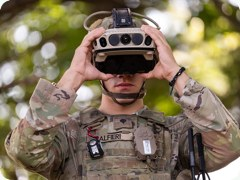
\includegraphics[height=13mm]{app_mr.jpg}\\[1pt]
    C.1 Tactical mixed reality under cognitive attack
  \end{minipage}\hfill
  \begin{minipage}[t]{0.235\linewidth}\centering
    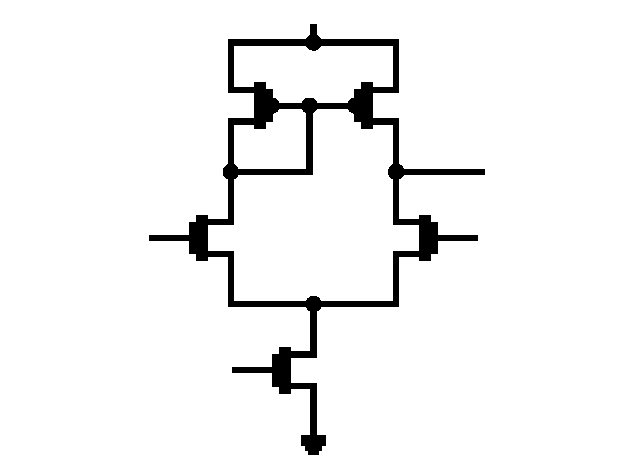
\includegraphics[height=13mm]{app_ic_ota.pdf}\\[1pt]
    C.2 Analog circuit design
  \end{minipage}\hfill
  \begin{minipage}[t]{0.235\linewidth}\centering
    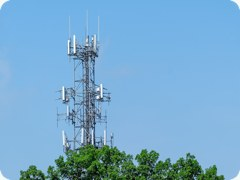
\includegraphics[height=13mm]{app_oran.jpg}\\[1pt]
    C.3 Open radio access networks
  \end{minipage}\hfill
  \begin{minipage}[t]{0.235\linewidth}\centering
    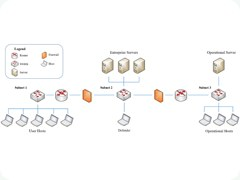
\includegraphics[height=13mm]{app_cage.jpg}\\[1pt]
    C.4 Autonomous cyber defense
  \end{minipage}\\[3pt]
  {\centering\textbf{\normalsize (C) Deployed Systems: Where the Guarantees Are Enforced}\par}};
\begin{pgfonlayer}{bg}
  \node[frame, draw=colC, dashed, fill=colC!5, fit=(A.west |- Ct.north) (B.east |- Ct.south)] (C) {};
\end{pgfonlayer}
% ---------- Arrows with verbs ----------
\draw[arr, colA] ([yshift=-6mm]A.north east) -- node[alab, text=colA, above] {Support} ([yshift=-6mm]B.north west);
\draw[arr, colC] ([xshift=22mm]C.north west) -- node[alab, text=colC, left] {Motivate} ([xshift=22mm]C.north west |- A.south);
\draw[arr, colB] ([xshift=-22mm]B.south east) -- node[alab, text=colB, right] {Enforce} ([xshift=-22mm]B.south east |- C.north);
\end{tikzpicture}
\end{document}
